%____________________________________________________________________________||
\section{Impact of shape based MC systematics} \label{app:sec_mc_based}

So far we only allowed correlated systematics, e.g. JEC, $b$-tags and more to vary the normalisation only in \MHT. 
In order to test possibly correlated effects on the \MHT variables we test the effect of adding MC based variation on the shape of \MHT not just on the normalisation. The study shows no significant effect on the limits. 


Figures~\ref{fig:mht_shape} shows the ratio of r-values obtained with and without MC based systematics applied on the \MHT shape discriminator. 

\begin{figure}[h!] \centering
  \subfigure{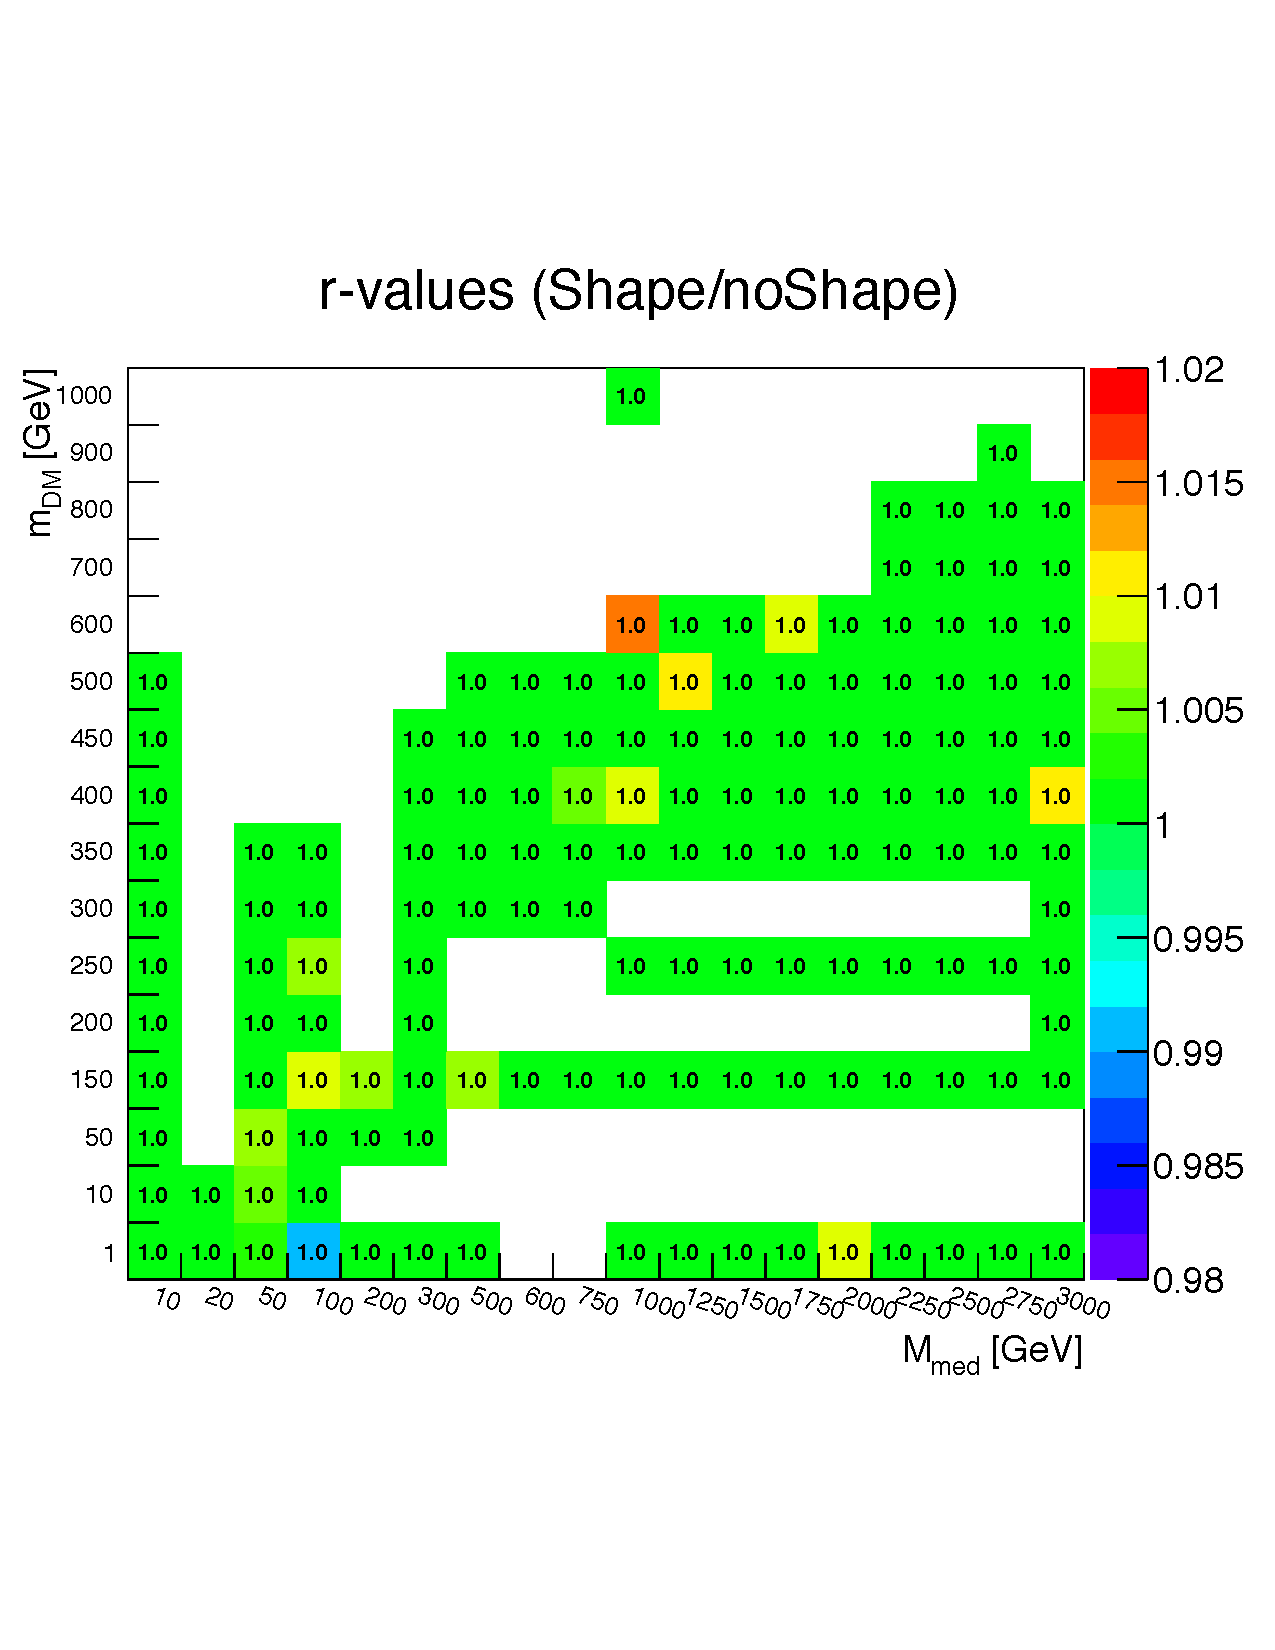
\includegraphics[width=0.4\textwidth]{figures/DMplots/ScorpionDMA_xs10_2p2fb_Shape_DIV_noShape__exp_r.pdf}}
  \subfigure{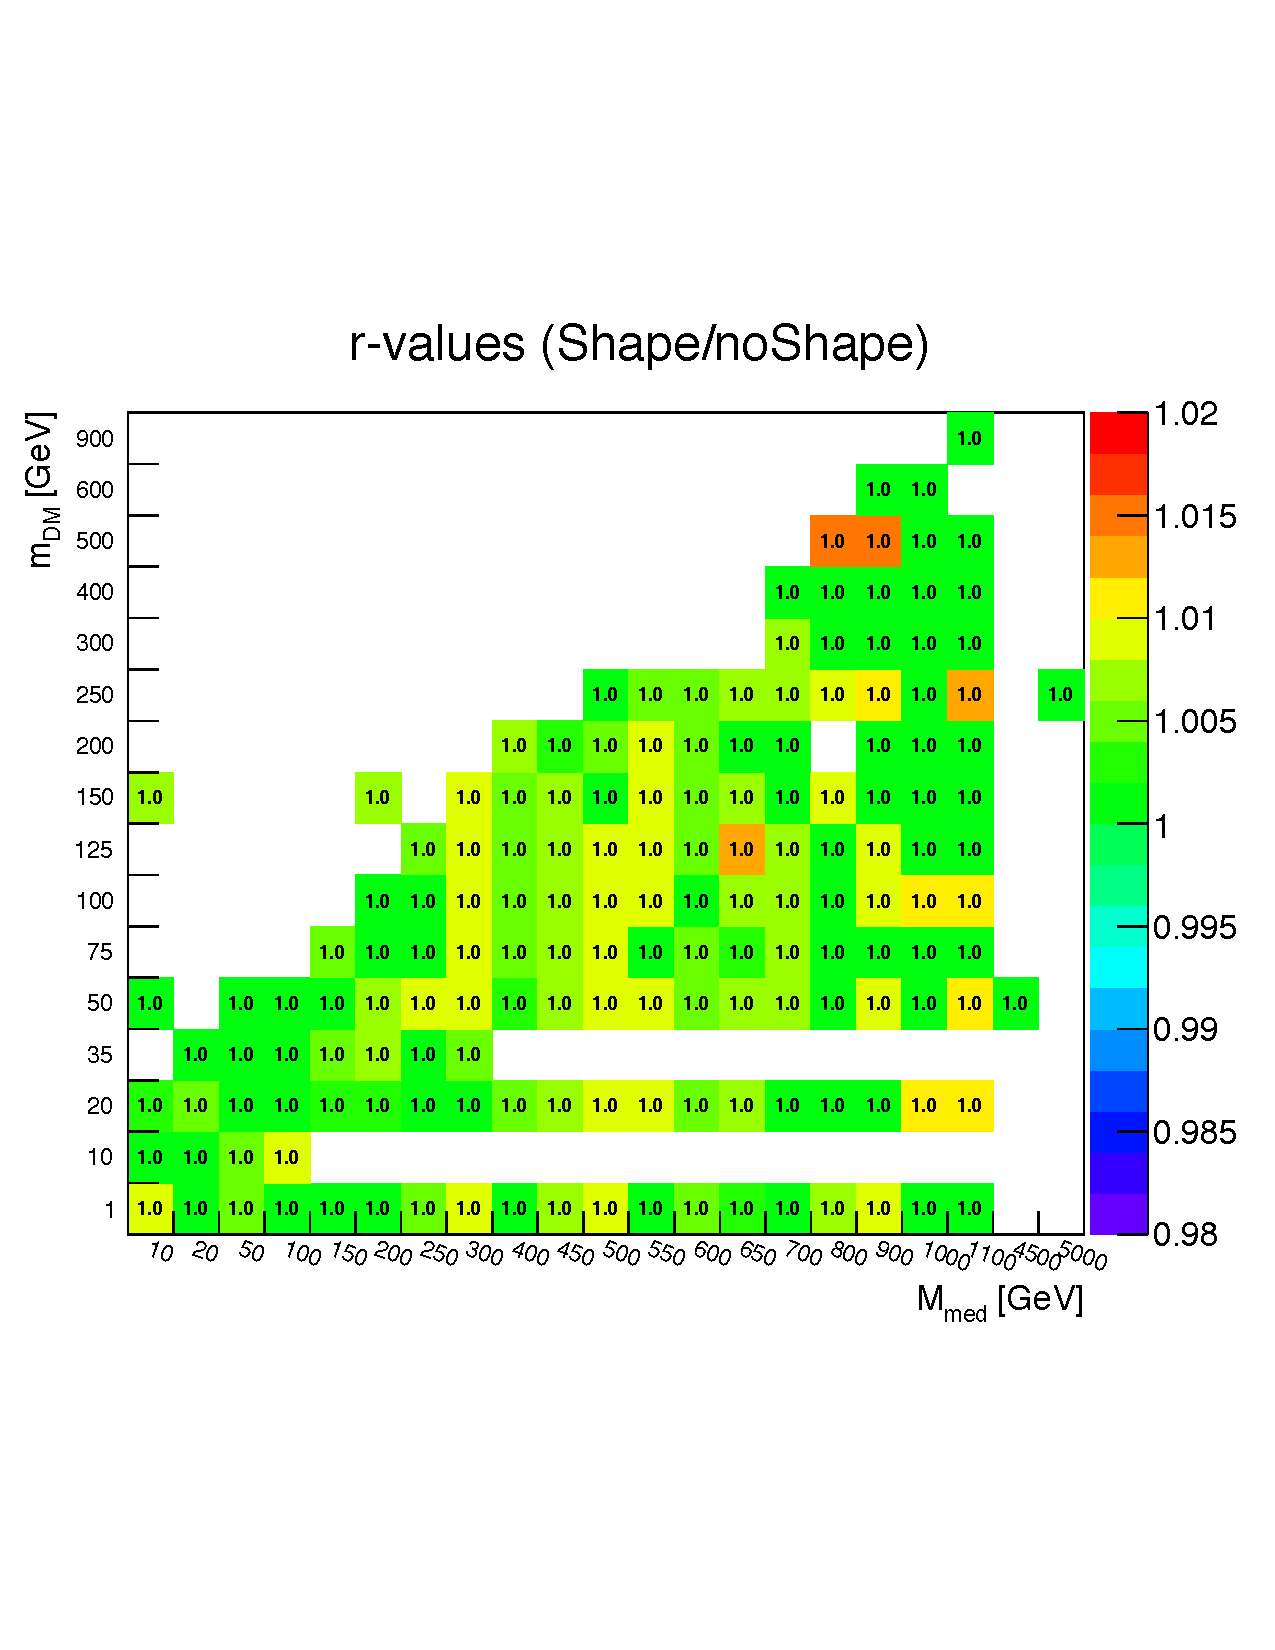
\includegraphics[width=0.4\textwidth]{figures/DMplots/ScorpionDMP_xs10_2p2fb_Shape_DIV_noShape__exp_r.pdf}}
  \caption{Ratio of r-values considering the MC based systematics as shape systematic for the axial vector model (left) and pseudoscalar model (right).}
\label{fig:mht_shape} 
\end{figure}

%\begin{figure}[h!] \centering
%  \subfigure{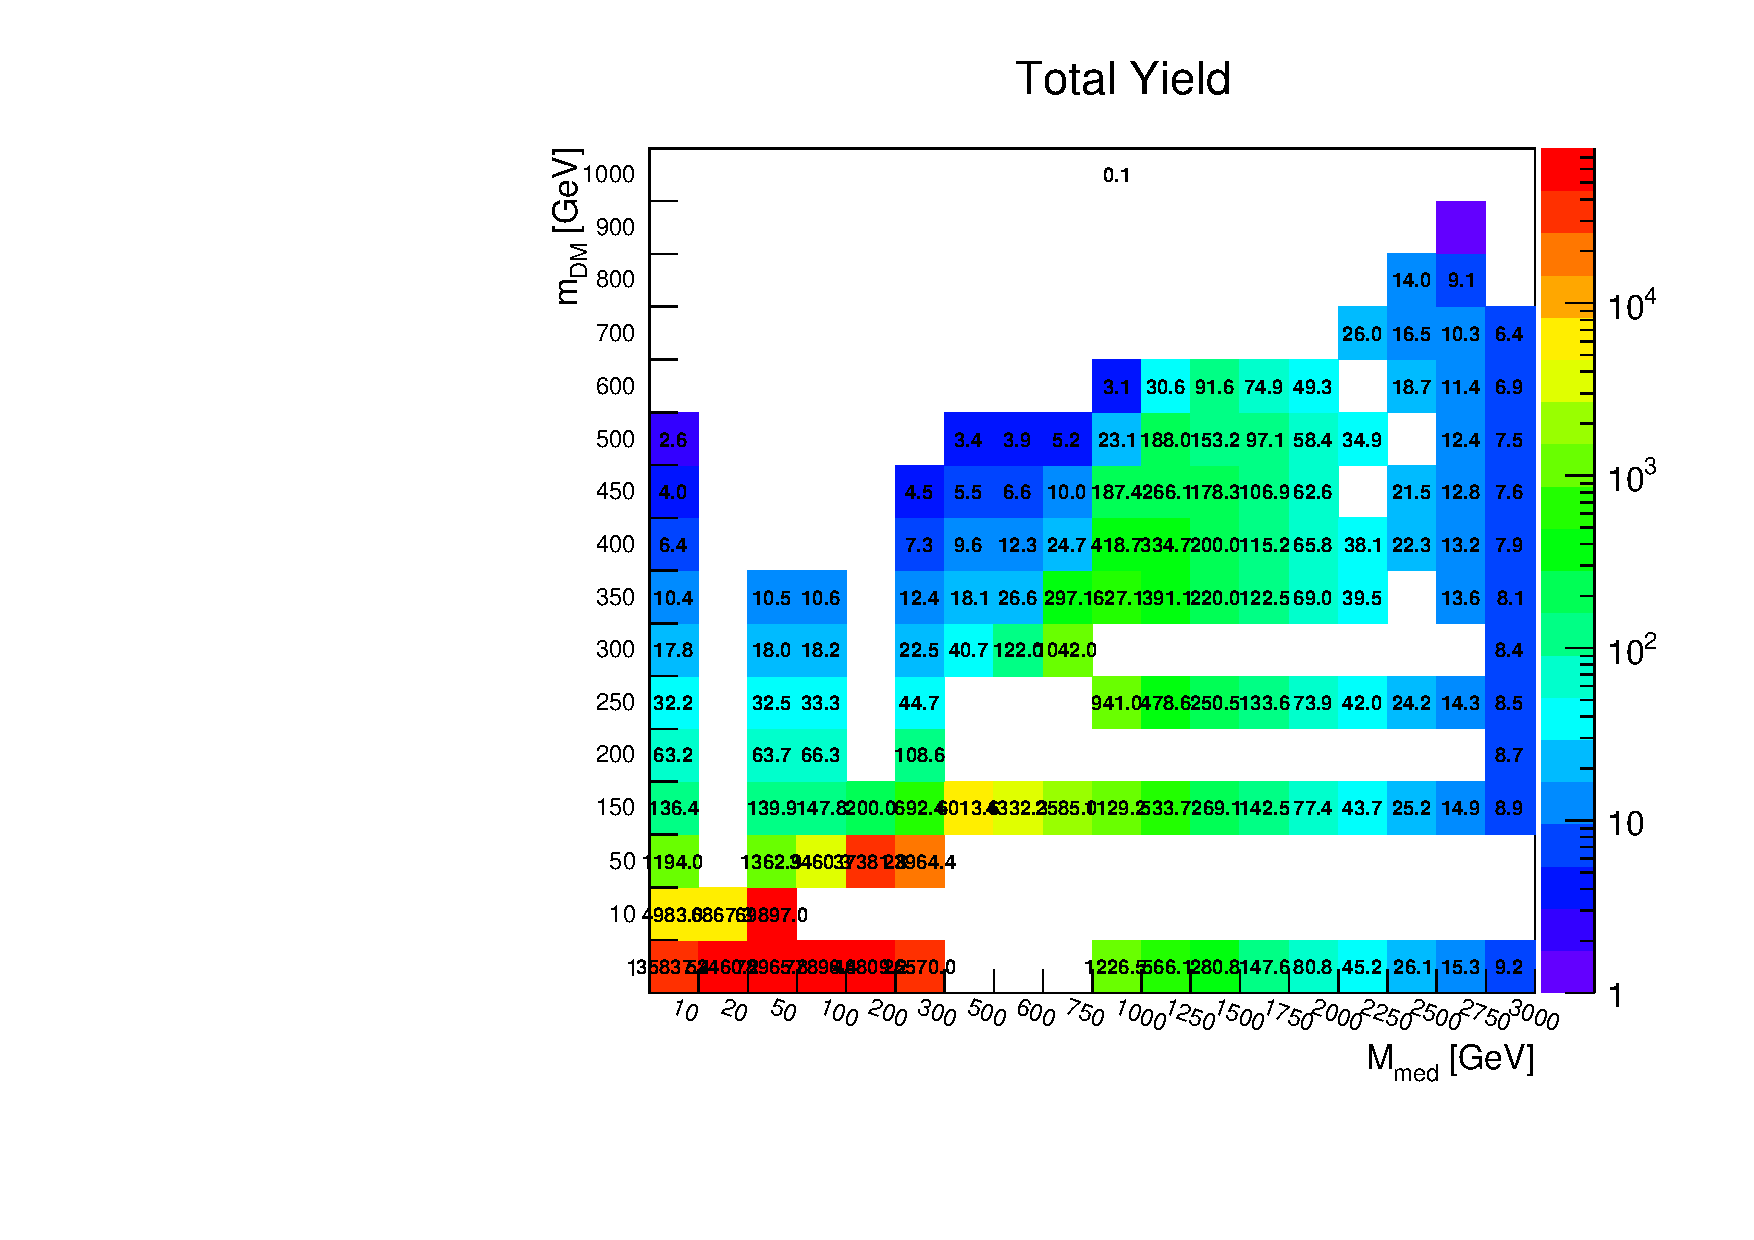
\includegraphics[width=0.35\textwidth]{figures/DMplots/SummaryPlot_ScorpionDMA_xs10_2p2fb_ShapeMCSyst_exp_yldTot.pdf}}
%  \subfigure{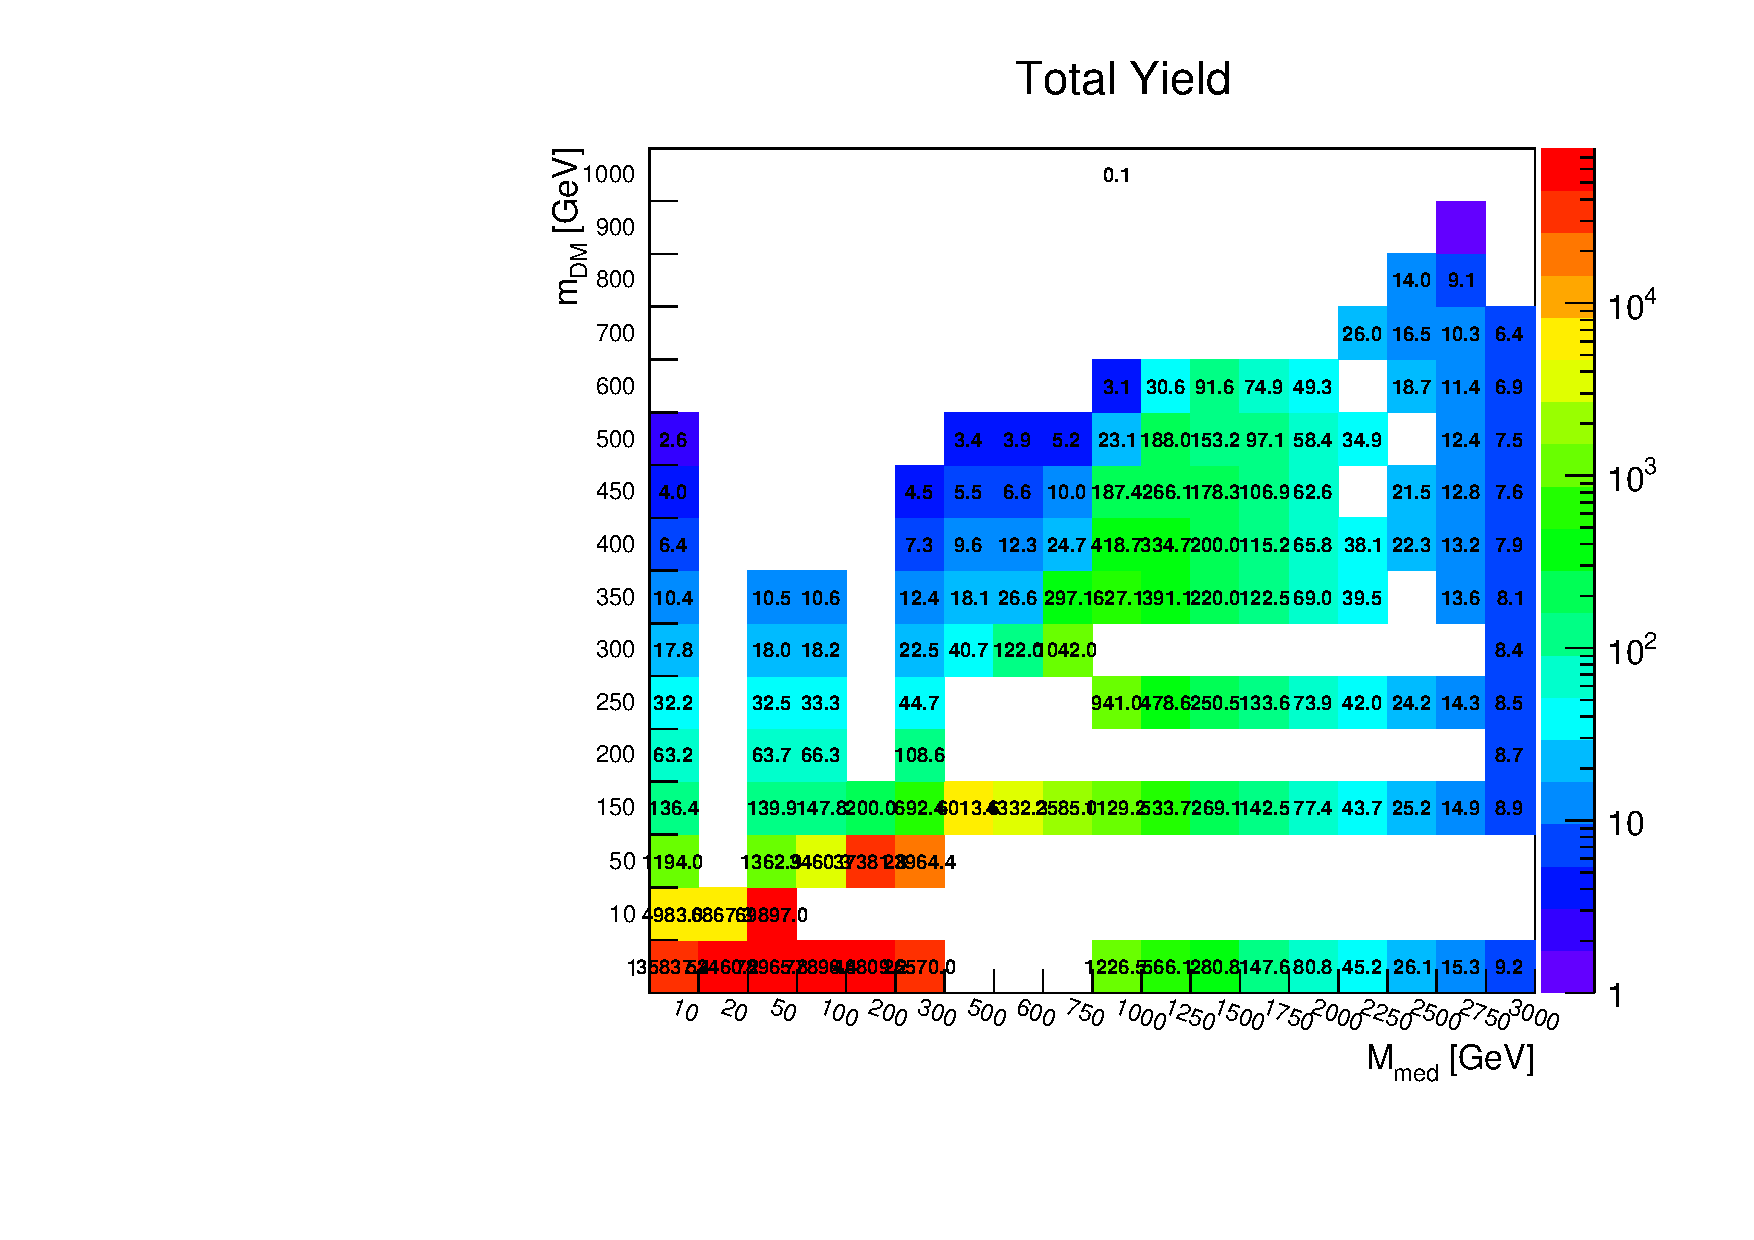
\includegraphics[width=0.35\textwidth]{figures/DMplots/SummaryPlot_ScorpionDMA_xs10_2p2fb_noShapeMCSyst_exp_yldTot.pdf}}
%  \subfigure{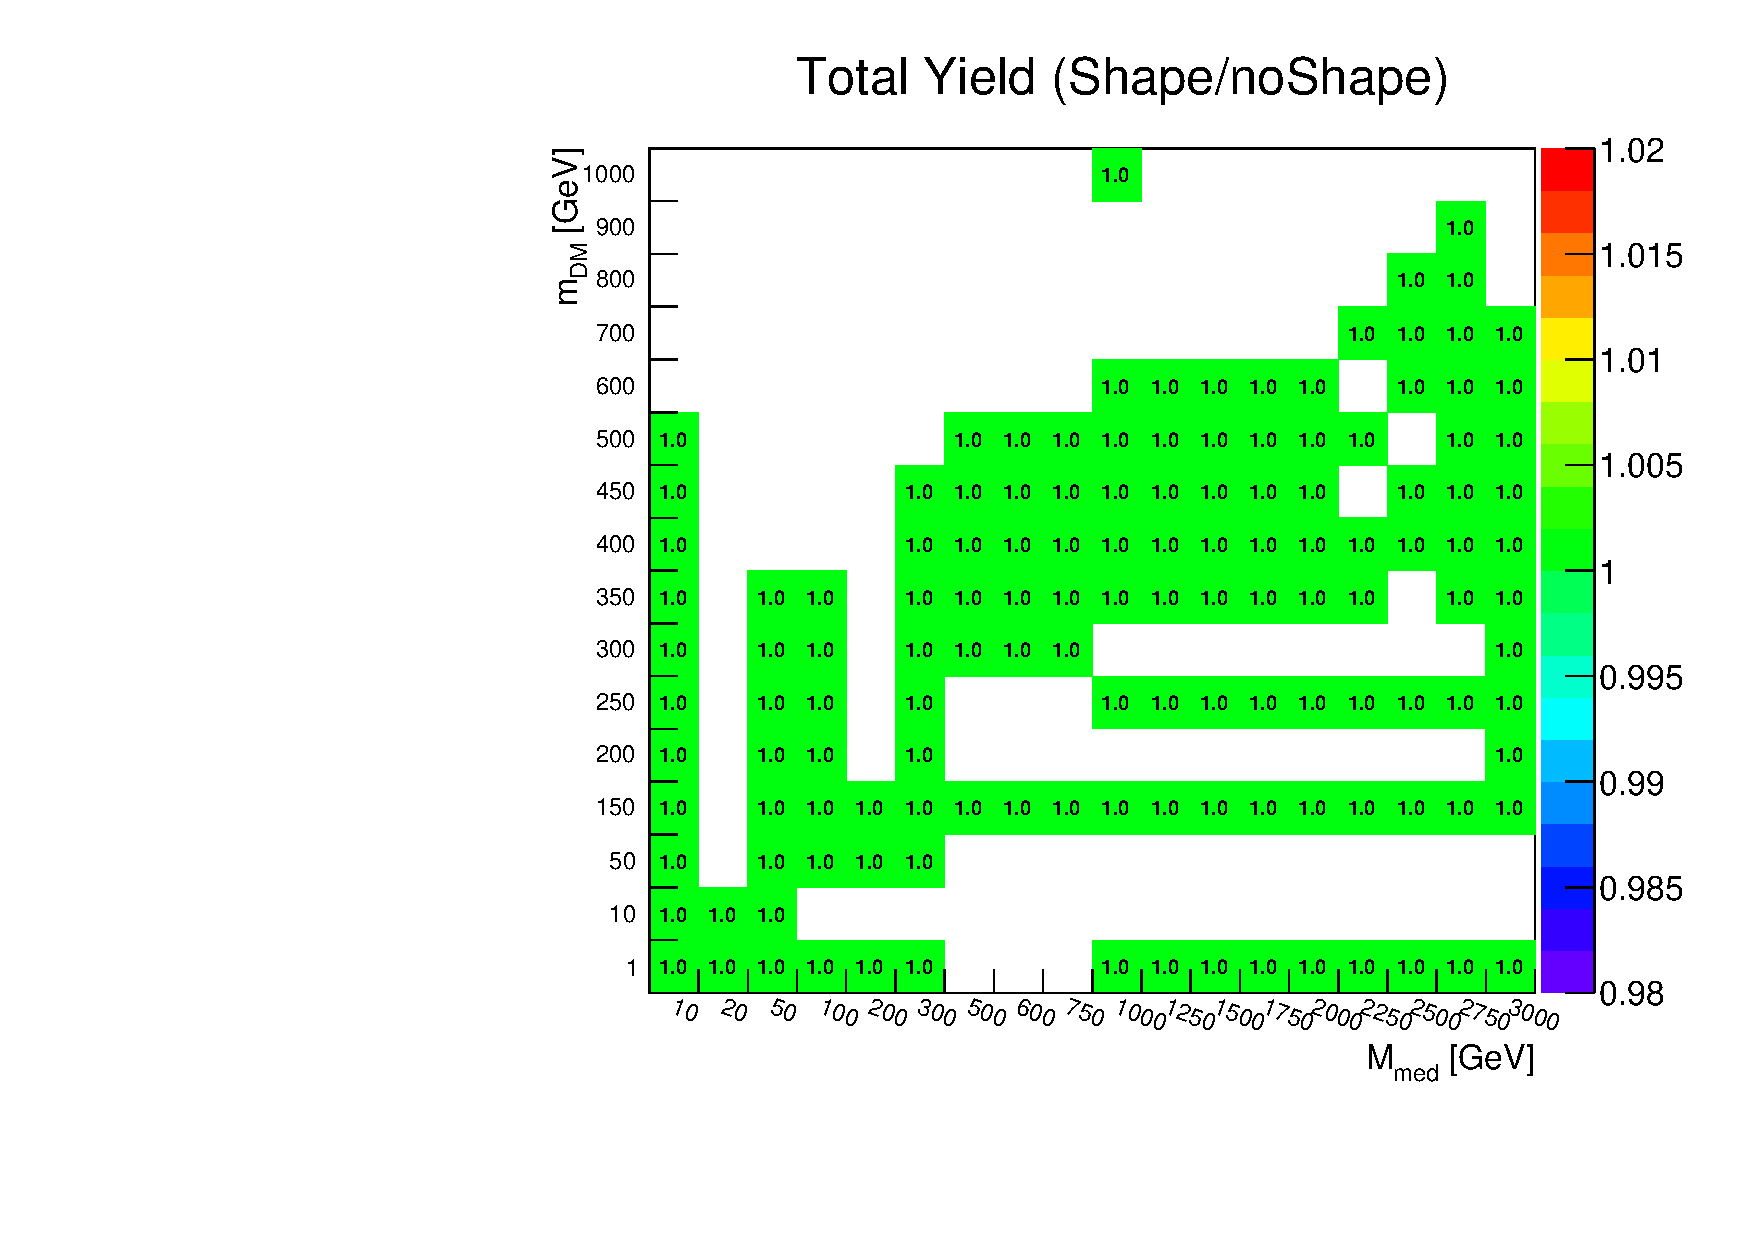
\includegraphics[width=0.35\textwidth]{figures/DMplots/ScorpionDMA_xs10_2p2fb_Shape_DIV_noShape__exp_yldTot.pdf}}
%  \caption{Differente between shape systematics considered (left), no shape systematics (middle) and their ratio (right) for axial-vector models.}}
%\label{fig:mht_shape_axial} 
%\end{figure}



%\begin{figure}[h!] \centeringe
%  \subfigure{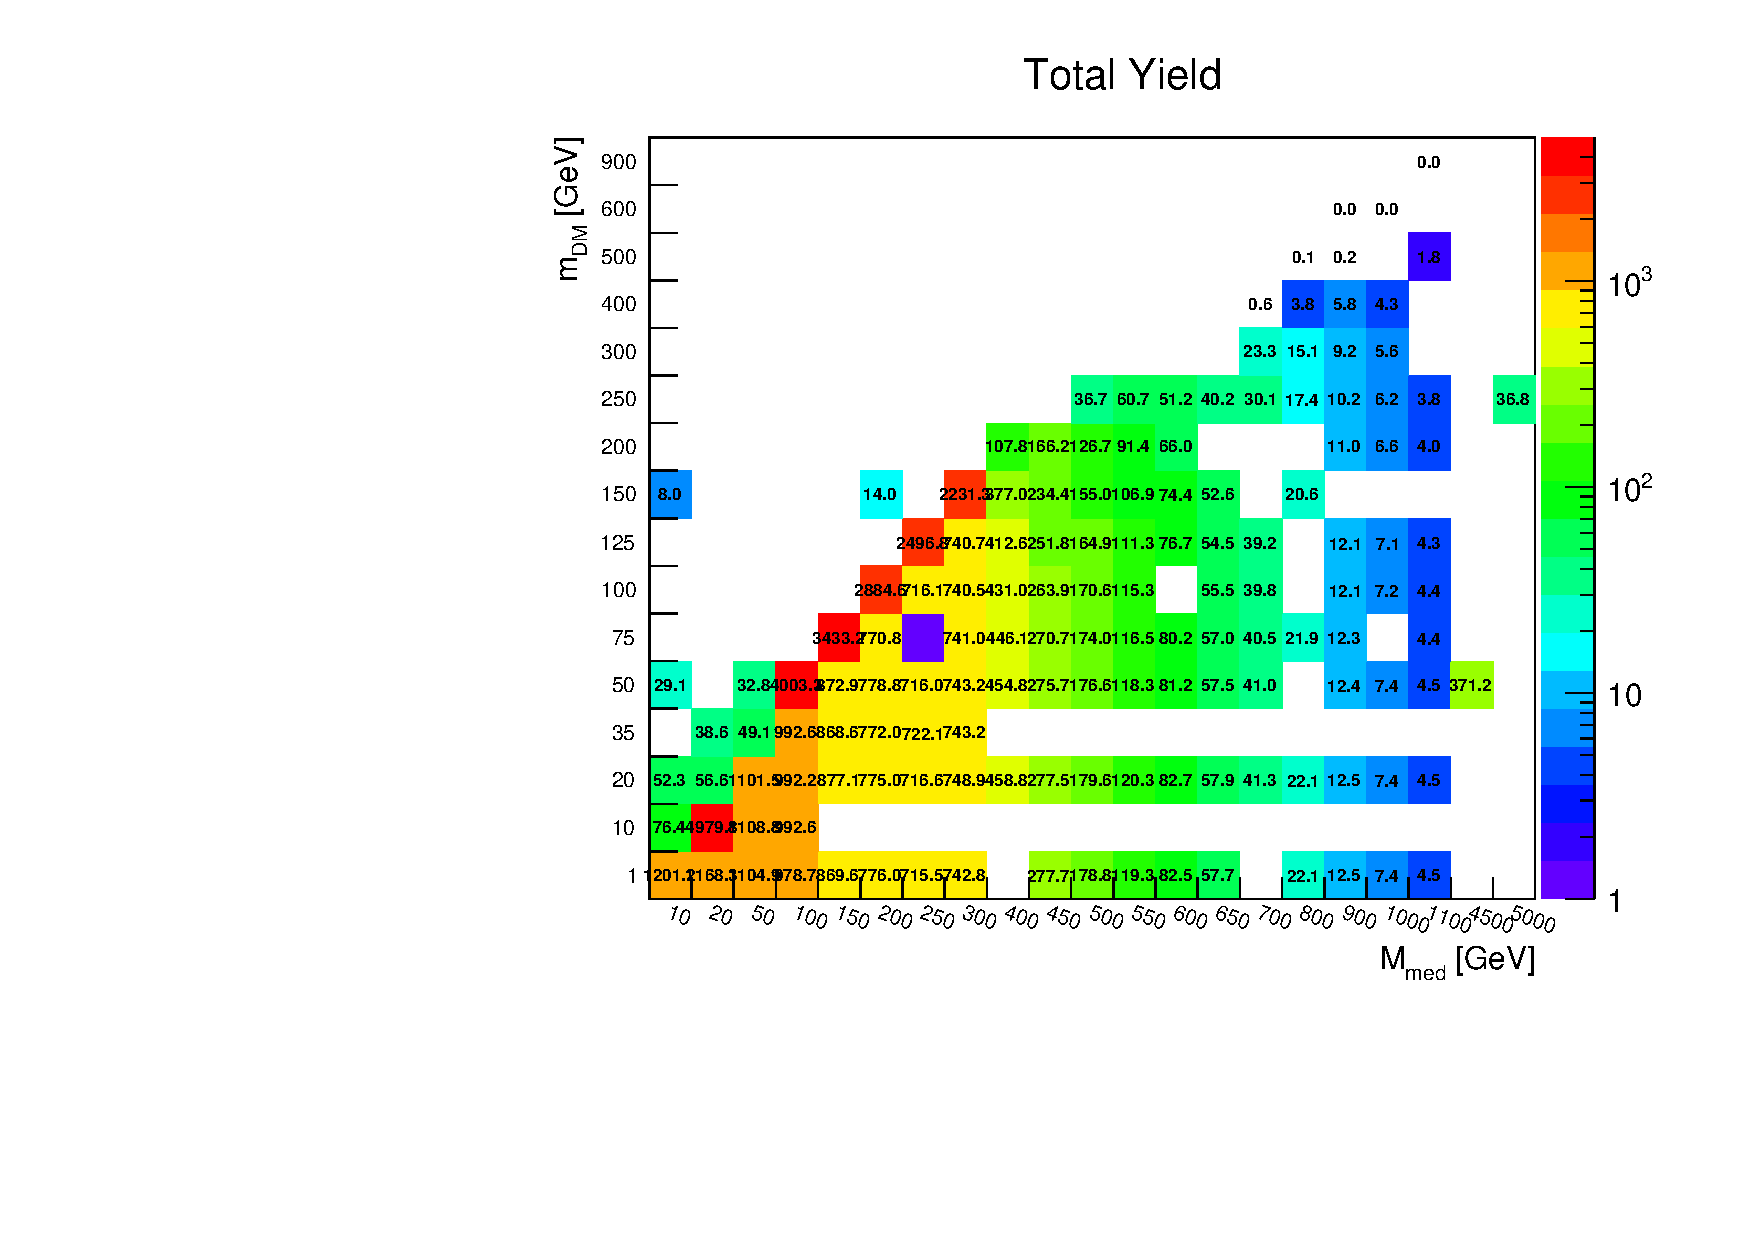
\includegraphics[width=0.35\textwidth]{figures/DMplots/SummaryPlot_ScorpionDMP_xs10_2p2fb_ShapeMCSyst_exp_yldTot.pdf}}
%  \subfigure{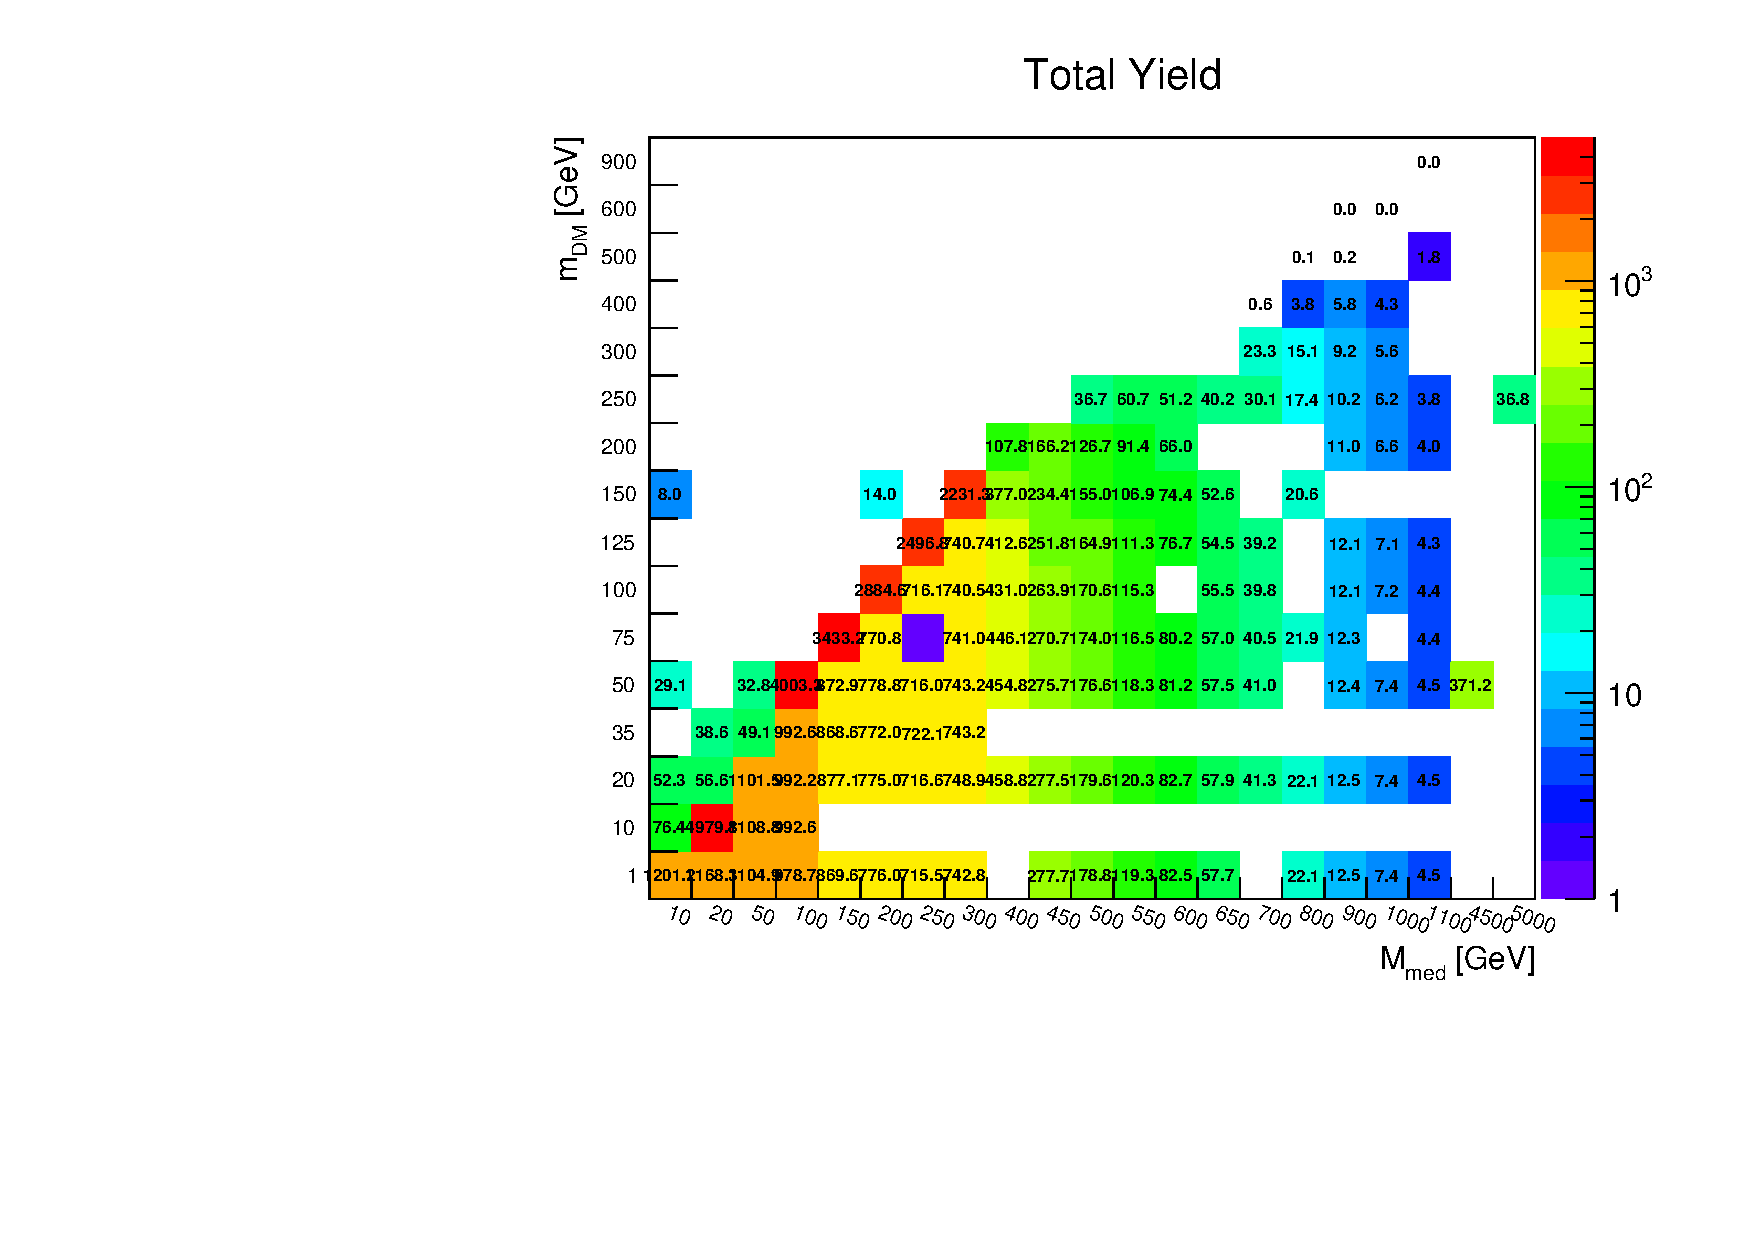
\includegraphics[width=0.35\textwidth]{figures/DMplots/SummaryPlot_ScorpionDMP_xs10_2p2fb_noShapeMCSyst_exp_yldTot.pdf}}
%  \subfigure{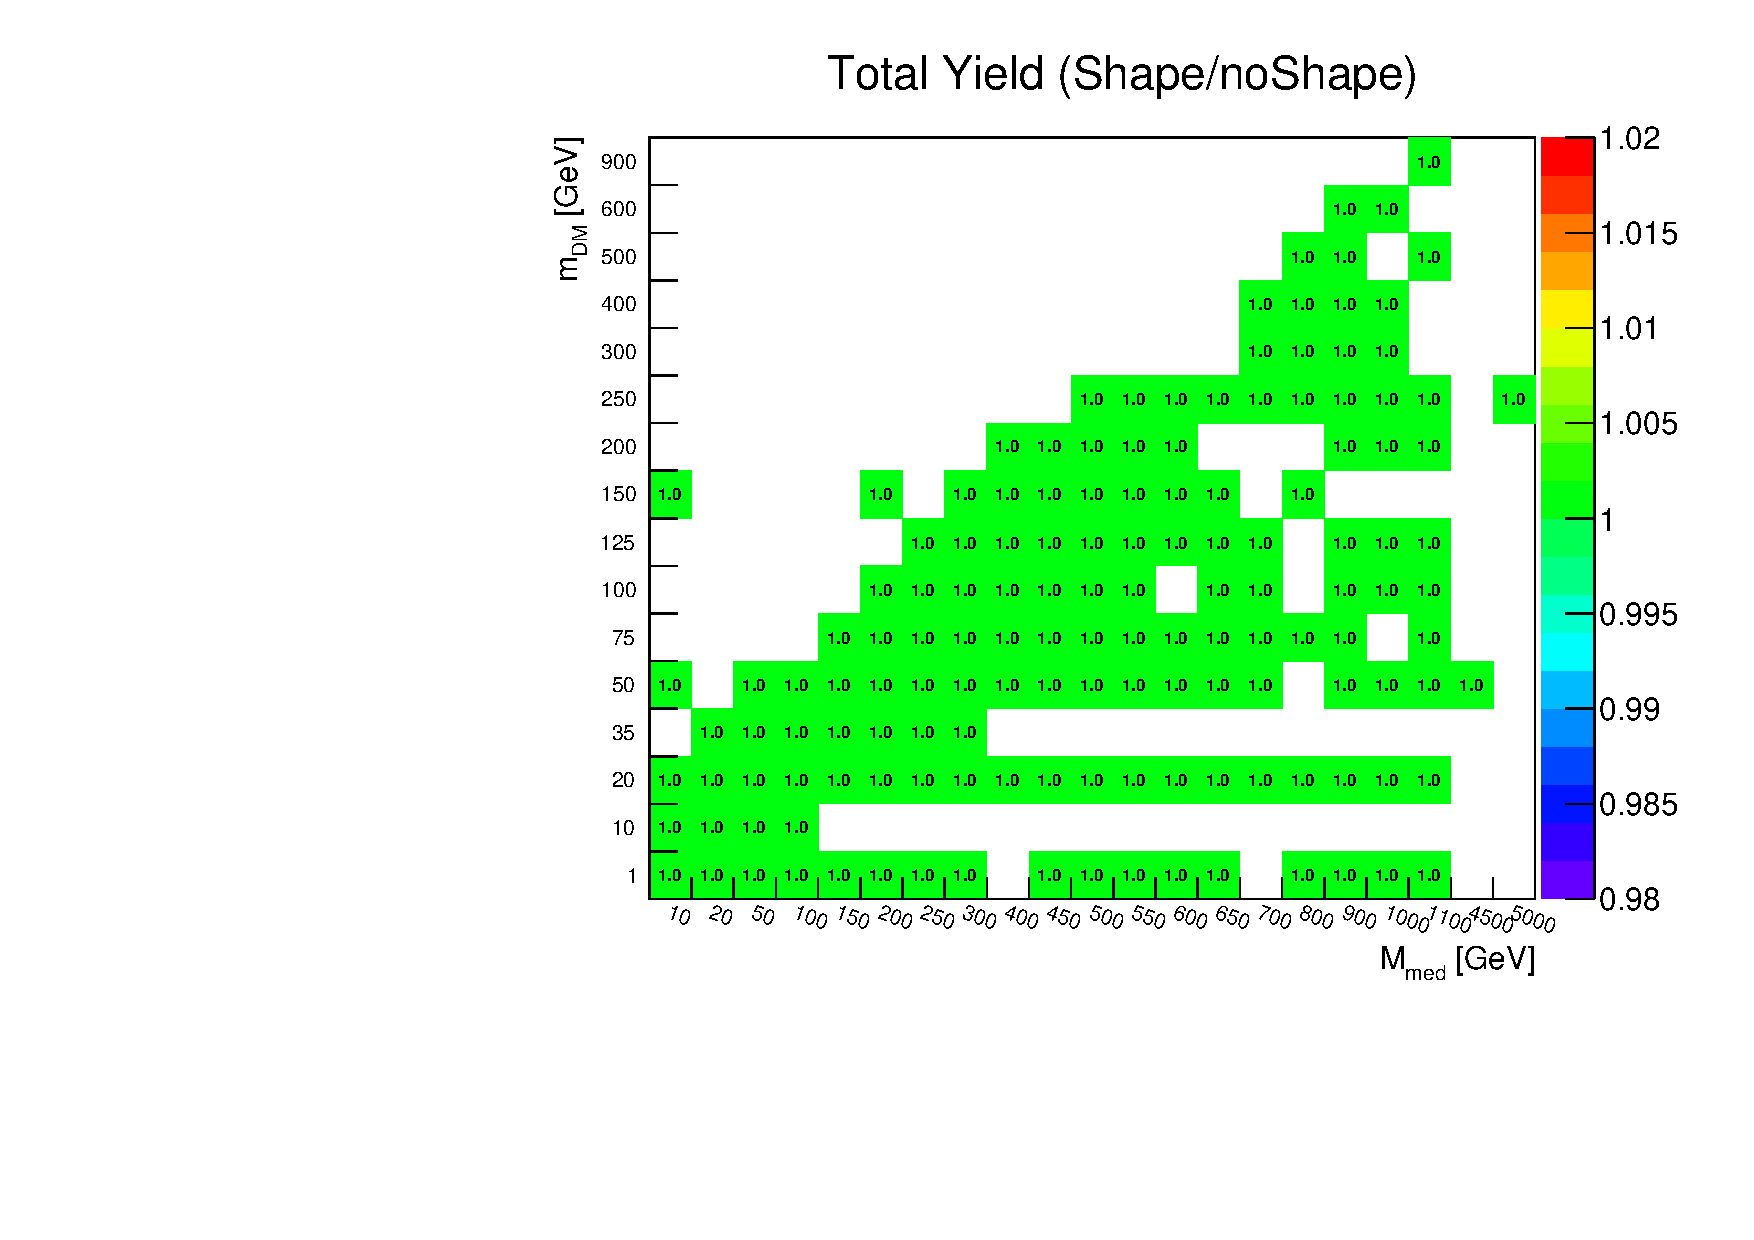
\includegraphics[width=0.35\textwidth]{figures/DMplots/ScorpionDMP_xs10_2p2fb_Shape_DIV_noShape__exp_yldTot.pdf}}
%  \caption{Differente between shape systematics considered (left), no shape systematics (middle) and their ratio (right) for scalar models.}}
%\label{fig:mht_shape_scalar} 
%\end{figure}

\section{Higher order corrections}
%The RA1 analysis is designed to be robust to missing higher order corrections in MC. The normalisations in each $H_{T}, N_{j}, N_{b}$ bin are taken from control regions binn

On request from the MET+X conveners, we evaluated the impact of higher order 
corrections on our analysis. The LO MC for the V+jets processes was reweighted 
according to corrections provided by the monojet group that account for higher 
order QCD and EWK corrections as a function of boson \Pt \cite{Monojet:AN2015-072}. The effect of these 
corrections on our transfer factors to estimate the backgrounds are 
shown in Tab.~\ref{tab:nloBosonPt}. The table shows the ratio of the transfer factor calculated 
with and without applying these corrections, shown separately for QCD only and 
QCD+EWK. They have a small impact on our transfer factor for the monojet bin 
where studying the effect of these corrections is most applicable. The small few \% effect observed is well covered by the systematic uncertainty on the 
transfer factor obtained from closure tests, which ranges from 10-30\% for the 
$\gamma$ to $Z$ ratio and 10-30\% for the $W$ to $Z$ ratio. 


\begin{table}
\tiny
\centering

\begin{tabular}{cccccccc}
\hline\hline
& \multicolumn{8}{c}{\scalht (\gev)}\\
Transfer factor & 200-250 & 250-300 & 300-350 & 350-400 & 400-500 & 500-600 & 600-800  \\
$\mu \rightarrow W$ & $0.99\pm0.04$ & $0.99\pm0.03$ & $0.00\pm0.02$ & $0.99\pm0.02$ & $0.98\pm0.02$ & $0.99\pm0.02$ & $0.98\pm0.03$ \\
$\mu\mu \rightarrow Z$ & $1.00\pm0.04$ & $1.00\pm0.03$ & $0.99\pm0.02$ & $1.00\pm0.02$ & $0.99\pm0.02$ & $0.98\pm0.02$ & $0.99\pm0.03$  \\
$\mu \rightarrow Z$ & $1.00\pm0.04$ & $0.99\pm0.03$ & $1.00\pm0.02$ & $1.00\pm0.02$ & $1.01\pm0.02$ & $1.01\pm0.03$ & $1.02\pm0.03$  \\
$\gamma \rightarrow Z$ & - & - & - & - & $1.01\pm0.03$ & $0.99\pm0.03$ & $0.95\pm0.03$  \\
\hline\hline
\end{tabular}

\\ \vspace{5mm}

\begin{tabular}{cccccccc}
\hline\hline
& \multicolumn{8}{c}{\scalht (\gev)}\\
Transfer factor & 200-250 & 250-300 & 300-350 & 350-400 & 400-500 & 500-600 & 600-800  \\
$\mu \rightarrow W$ & $0.99\pm0.04$ & $0.99\pm0.03$ & $0.99\pm0.02$ & $0.98\pm0.02$ & $0.98\pm0.02$ & $1.00\pm0.02$ & $1.01\pm0.03$  \\
$\mu\mu \rightarrow Z$ & $0.99\pm0.04$ & $1.00\pm0.03$ & $0.99\pm0.02$ & $1.00\pm0.02$ & $0.99\pm0.02$ & $0.98\pm0.02$ & $0.99\pm0.03$  \\
$\mu \rightarrow Z$ & $1.00\pm0.04$ & $0.99\pm0.03$ & $1.01\pm0.03$ & $1.01\pm0.02$ & $1.02\pm0.02$ & $1.03\pm0.03$ & $1.05\pm0.03$  \\
$\gamma \rightarrow Z$ & - & - & - & - & $1.01\pm0.03$ & $0.98\pm0.03$ & $0.93\pm0.03$  \\
\hline\hline
\end{tabular}


\caption{Ratio of transfer factors with/without boson \Pt-dependent QCD NLO (top) and QCD+EWK NLO (bottom) corrections for the monojet category. }
\label{tab:nloBosonPt}
\end{table}




